\documentclass[uplatex]{jsarticle}

\input{setting}
\title{格子ボルツマン法による変化球軌道シミュレーション\\--- 理論と実装 ---}
\author{TODO: 著者名を記入}

\begin{document}
\maketitle
\tableofcontents

\newpage
\section{はじめに}
\label{sec:intro}

野球における変化球の軌道は，リリース時の球速・回転数・回転軸の向き，および球体表面の縫い目の位置によって決まる空気力学的な力（抗力・揚力・非マグヌス力）の積分として定まる。
なかでも縫い目まわりの流れの剥離点が回転軸方向に応じて非対称に移動することで生じる非マグヌス力は，スウィーパーに代表される近年の変化球の大きな変化量を説明する要因のひとつと考えられているが，その大きさは風洞実験や実測データからの間接的な推定に頼っており，流体の詳細な挙動そのものを直接観測することは難しい。

本ノートは，格子ボルツマン法（Lattice Boltzmann Method, LBM）による3次元非定常流体解析と，ボールの並進・回転運動を記述する剛体力学とを1ステップごとに結合する数値シミュレーションにより，縫い目付き球体まわりの乱流場とそれが生成する軌道を再現することを目的とするプロジェクトの，理論的背景と実装方法をまとめたものである。

\subsection{LBMを採用する理由}

対象とする流れは，ボール直径程度の代表長さに対してレイノルズ数が\(10^5\)のオーダーに達する乱流であり，かつ球体表面の縫い目という数ミリメートル規模の幾何学的特徴が剥離点の位置を左右する。
このような問題に対しては，
\begin{itemize}
	\item 移動・回転する複雑形状境界を陽に扱いやすいこと，
	\item 各格子点の更新が局所的な演算のみで完結し，GPUによる大規模並列化と親和性が高いこと，
	\item 圧縮性ナビエ・ストークス方程式を弱圧縮性極限で近似的に解くことで，非定常な渦構造を陽に解像できること，
\end{itemize}
の3点から，格子ボルツマン法を採用した。
特にGPUによる並列計算との親和性は，1球の投球について本塁到達までの飛行時間（約0.5秒）を3次元乱流解析として計算する上で実用上の制約となる計算コストを扱える範囲に収めるために不可欠である。

\subsection{密結合方式によるボールとの相互作用}

ボールに働く力とトルクは流体解析から瞬時に決まり，その力とトルクがボールの並進・回転運動を変化させ，運動が変化した結果として境界条件が更新され，それが次の瞬間の流体解析に影響する。
本プロジェクトでは，この双方向の依存関係を近似せずに毎ステップ解くという意味で，これを「密結合方式」と呼んでいる。
具体的には，ボールを常に計算領域の中心に固定した「ボール追従座標系」を採用し，ボールの並進運動を計算領域全体に課す一様な体積力（非慣性系の見かけの力）として実現することで，領域を移動させることなく長距離の飛行を計算できるようにしている。
密結合方式の詳細な導出は\secref{coupling}で述べる。

\subsection{本ノートの構成}

本ノートは，開発の過程で得られた検証結果や設計判断を随時記録している設計ノート（本リポジトリの\texttt{docs/design/DESIGN.md}）をもとに，理論と実装の要点を整理し直したものである。構成は次のとおりである。

\begin{itemize}
	\item \secref{aerodynamics}：野球ボールの空気力学的背景（無次元パラメータ，抗力，マグヌス力・非マグヌス力，運動方程式）
	\item \secref{lbm}：格子ボルツマン法の基礎理論（ボルツマン方程式，離散速度セット，格子単位系）
	\item \secref{cumulant}：数値的安定性のための中心モーメント衝突演算子
	\item \secref{turbulence}：乱流モデリング（LES，Smagorinskyモデル，壁面近傍の扱い）
	\item \secref{geometry-boundary}：縫い目形状のパラメトリックモデリングと移動境界条件
	\item \secref{coupling}：ボールとの密結合による軌道計算アルゴリズム
	\item \secref{gpu}：GPUによる並列実装
	\item \secref{validation}：解析解・実験値との比較による検証（Validation \& Verification）
\end{itemize}


\newpage
\section{野球ボールの空気力学的背景}
\label{sec:aerodynamics}

本章では，投球中の野球ボールに働く空気力学的な力を特徴づける無次元パラメータと，本プロジェクトが対象とする物理現象——縫い目に起因する非マグヌス力——について整理する。

\subsection{基本諸元と支配的な無次元パラメータ}
\label{sec:aero-params}

公式野球ボールの直径は円周の規定（9.00--9.25\,in）から72.9--74.9\,mmであり，本プロジェクトでは中央値 \(D = 0.0748\,\text{m}\) を既定値としてパラメータ化する。質量は既定 \(m = 0.145\,\text{kg}\)。表面には108個の二重縫い目からなる1本の連続曲線が球面上を二重らせん状に周回しており，その凸高さは実測で平均約0.79\,mm（\(D/92\) 程度）と報告されている\cite{kensrud2010thesis}。

\paragraph{2シーム・4シームについての注記}
野球ボールの縫い目は幾何学的には1種類（108個の二重縫い目からなる単一の閉曲線）しか存在しない。投げ方（グリップ）によって変わるのは，\emph{この固定された縫い目パターンに対する回転軸の向きと位相}である。回転軸をある向きに取ると1回転あたり4本の縫い目が気流を横切るように見え，別の向きでは2本に見える——これが「4シーム」「2シーム」という分類の正体であり，別々の幾何形状ではない。したがって本プロジェクトでは縫い目曲線を1つだけ実装し，投球条件として「回転軸の向き（チルト角・ヨー角）」と「縫い目パターンに対する初期位相角」を与える設計とする（\secref{seam-geometry}）。

代表投球速度は \(U = 20\)--45\,m/s，代表回転数は1500--3500\,rpmである。これらから定まる無次元パラメータのうち，本問題の物理を支配する3つを挙げる。

\begin{itemize}
	\item \textbf{レイノルズ数} \(Re = UD/\nu\)。代表条件（\(U=40\,\text{m/s}\)，\(\nu_{air}\approx1.5\times10^{-5}\,\text{m}^2/\text{s}\)）で \(Re\approx2.0\times10^5\)。文献では投球速度域で \(Re\approx1.1\text{--}2.4\times10^5\) と報告される\cite{nathan2008,kensrud2010thesis}。この値は滑面球の臨界レイノルズ数（ドラッグクライシス）が生じる遷移域に重なるため，境界層の層流--乱流遷移の位置が抗力に敏感に効く。
	\item \textbf{スピンパラメータ} \(S = \omega r/U\)（\(\omega\)：角速度，\(r\)：半径）。実投球では \(S\approx0.09\text{--}0.6\) 程度。
	\item \textbf{マッハ数} \(Ma = U/c\)。\(0.15\) 以下では圧縮性の影響は小さいが，格子ボルツマン法は元来弱圧縮性モデルであるため，格子単位系の設計において格子マッハ数を明示的に管理する必要がある（\secref{lattice-units}）。
\end{itemize}

\subsection{抗力とドラッグクライシス}

滑らかな球では，境界層が層流のまま剥離する亜臨界域で \(C_D\approx0.5\) 程度と大きいが，\(Re\) が臨界値を超えると境界層が乱流に遷移して剥離点が後方へ移動し，\(C_D\) が急減する（drag crisis）。

野球ボールでは縫い目が人工的な乱流トリップとして働くため，滑面球のような急峻なドラッグクライシスは示さず，縫い目の向きに依存してなだらかかつ非対称に \(C_D\) が変化することが実験的に確認されている\cite{kensrud2010thesis,kensrud2017study}。したがって本シミュレーションでは，滑面球の近似ではなく\emph{縫い目形状を含めた表面ジオメトリで境界層遷移・剥離を直接解像する}方針をとる。

後述するように，本プロジェクトの代表条件では縫い目の凸高さと層流境界層厚がほぼ一致する（\secref{resolution-budget}）。粗さ要素が境界層と同程度の高さを持つことは，それが遷移を誘発するトリップとして機能する条件そのものであり，縫い目を解像することと境界層を解像することは実質的に1つの要求である。

\subsection{マグヌス力と非マグヌス力（縫い目由来の横力）}
\label{sec:magnus}

回転する球のまわりでは，回転方向側の境界層が加速されて剥離が遅れ，反対側では剥離が早まることで循環が生じ，進行方向に垂直な力（マグヌス力）が発生する：
\begin{align}
	F_L = \frac{1}{2}\rho U^2 A\, C_L(S, Re, \text{seam orientation}).
	\label{eq:magnus}
\end{align}
実験的には \(S<0.4\) 程度の範囲で \(C_L\approx S\)（傾き1の線形関係）が良い近似となる\cite{nathan2008,lyu2011dragspin}が，この関係は滑面球の理想解に対する近似である。実際の野球ボールでは，縫い目の向きによって主流に対して非対称な圧力分布が生じ，マグヌス面（回転軸に直交する平面）から外れた方向の力——\textbf{非マグヌス力（横力）}——が発生することが知られている。これがスライダーやジャイロボール，スウィーパーが「教科書どおりの向きに曲がらない」現象の主要因である。

\textbf{本コードの設計要件}は，簡略化されたマグヌス力の解析式を用いるのではなく，縫い目形状を含む球体表面を境界条件として直接解像し，抗力係数 \(C_D\)・マグヌス方向の揚力係数 \(C_L\)・非マグヌス方向の横力係数 \(C_{side}\) をすべて流体場から直接算出することである。力の分解方法は\secref{coupling-loop}で述べる。

\subsection{運動方程式}
\label{sec:eom}

質量中心の並進運動：
\begin{align}
	m\frac{d\vec V}{dt} = \vec F_{drag} + \vec F_{Magnus} + \vec F_{side} + m\vec g.
	\label{eq:translation}
\end{align}
回転運動（角速度減衰，ジャイロ効果を含む一般形）：
\begin{align}
	I\frac{d\vec\omega}{dt} = \vec T_{aero}.
	\label{eq:rotation}
\end{align}
投球中の回転数減衰は数\%程度と小さいが，トルクは流体場から評価できる設計とする。本プロジェクトの密結合方式（\secref{coupling}）では，この運動方程式は係数テーブルではなく，CFDから毎ステップ得られる瞬時の力・トルクを直接使って積分する。


\newpage
\section{格子ボルツマン法の基礎理論}
\label{sec:lbm}

\subsection{ボルツマン方程式とBGK近似}

格子ボルツマン法（Lattice Boltzmann Method, LBM）は，Navier-Stokes方程式を直接離散化するのではなく，より基礎的な運動論レベルの方程式——ボルツマン輸送方程式——から出発し，Chapman-Enskog展開によってマクロスケールで圧縮性の弱いNavier-Stokes方程式を導出するアプローチである。

分子速度分布関数 \(f(\vec x,\vec\xi,t)\) に対するボルツマン方程式を，単一緩和時間（BGK）近似で時間・空間・速度空間すべてについて離散化すると次の格子ボルツマン方程式を得る：
\begin{align}
	f_i(\vec x+\vec e_i\Delta t,\ t+\Delta t) - f_i(\vec x,t)
	= -\frac{1}{\tau}\left[f_i(\vec x,t) - f_i^{eq}(\vec x,t)\right],
	\label{eq:lbe}
\end{align}
ここで \(f_i\) は離散速度方向 \(i\) の分布関数，\(\vec e_i\) は格子速度ベクトル，\(\tau\) は無次元緩和時間，\(f_i^{eq}\) はMaxwell-Boltzmann分布の低マッハ数展開である局所平衡分布である。緩和時間は動粘性係数と
\begin{align}
	\nu = c_s^2\left(\tau - \frac{1}{2}\right)\Delta t
	\label{eq:viscosity}
\end{align}
の関係で結びつく。ここで \(c_s = 1/\sqrt3\)（格子単位）は格子音速である。\eref{lbe}の右辺で表される衝突ステップと，左辺の並進（ストリーミング）ステップはいずれも局所演算のみで構成され，格子点間の通信は最近傍への値のコピーに限られる。この局所性が，GPUによる大規模並列化との親和性の根拠である。

\subsection{離散速度セット}

本プロジェクトでは2つの離散速度セットを用いる。

\begin{itemize}
	\item \textbf{D3Q19}：標準的な3次元計算に用いられるモデルで，メモリ効率と精度のバランスが良い。デバッグおよび低レイノルズ数での検証に用いる。
	\item \textbf{D3Q27}：本番計算（縫い目球・乱流）に用いる既定モデル。\secref{cumulant}で述べる中心モーメント衝突演算子は，D3Q27を必須とする——3次モーメント \(\sum_q w_q c_{x}^2c_{y}^2c_{z}^2\) がD3Q19では恒等的に0となる一方，D3Q27では \(c_s^6\) となり，3方向すべてに独立に分解できるのはD3Q27のみだからである。
\end{itemize}

本プロジェクトが対象とするレイノルズ数（\(Re\sim2\times10^5\)）は乱流域であり数値安定性が課題となるため，本番計算はD3Q27と中心モーメント衝突演算子の組を推奨構成とし，D3Q19+BGKは検証・軽量計算用の代替構成として残す。単一GPU（8\,GB VRAM）という制約下では，D3Q27はD3Q19よりメモリ使用量が増える点にも留意し，解像度とのトレードオフを\secref{resolution-budget}で検討する。

\subsection{格子単位系と物理量の変換}
\label{sec:lattice-units}

LBMは無次元格子単位（\(\Delta x=\Delta t=1\)）で計算するため，物理パラメータ（音速比・粘性・球速）を格子単位に変換する層が必要になる。設計上の要件は次の2点である。

\begin{itemize}
	\item 格子マッハ数 \(Ma_{lattice}=U_{lattice}/c_{s,lattice}\) を0.05--0.1程度に保つよう，代表速度と格子解像度から \(\Delta t\) を自動決定する。密結合方式（\secref{coupling}）では球速が飛行中にわずかに変化するため，初期速度を基準にマージンを持たせて設定する。
	\item 空間解像度 \(\Delta x\) はボール直径を何格子点で解像するか（\(N=D/\Delta x\)）で規定する。既定値は縫い目高さと境界層厚を何格子点で捉えるかという要件から決定する（\secref{resolution-budget}）。
\end{itemize}

一様な格子マッハ数で解像度を切る限り，格子粘性 \(\nu_{lattice}=\nu\,\Delta t/\Delta x^2\) は解像度 \(N\) に比例して大きくなる。したがって\emph{格子を細かくするほど \(\tau\) は\(1/2\)から離れて安定側に動く}——本プロジェクトの代表条件では，40点/Dで \(\tau-1/2=3.1\times10^{-5}\)，80点/Dで \(6.2\times10^{-5}\) となる。すなわち本番計算のコストを決めているのは数値安定性ではなく，飛行時間全体に必要なタイムステップ数である。


\section{衝突演算子と数値安定性}
\label{sec:cumulant}

単純なBGK（単一緩和時間）衝突演算子は，高レイノルズ数・低粘性域（\(\tau\to1/2\)）で数値不安定になりやすい。本番計算が要求する \(Re\sim2\times10^5\) では \(\tau-1/2\) が\(10^{-5}\)のオーダーとなるため，BGKでは実用にならない。本プロジェクトでは，安定性を確保するために\textbf{中心モーメント（キュムラント緩和）衝突演算子}を実装した（\texttt{src/core/central\_moments.jl}）。

\subsection{中心モーメント衝突演算子}

中心モーメント衝突演算子は，流体とともに動く座標系でモーメントを取り，その意味ごとに異なる緩和率を与える。

\begin{itemize}
	\item 2次モーメントの偏差成分（せん断応力を担う）は，動粘性を決める緩和率 \(\omega=1/\tau\) で緩和する。
	\item その対角和（トレース，音響＝体積粘性モード）は独立の緩和率 \(\omega_b\approx1\) で緩和する。これを2次の偏差成分と分離することが，安定性向上の主因である。
	\item 3次以上のモーメントは，キュムラントを0へ緩和する。これは「平衡値へ固定する」のとは異なり，\emph{その時点の2次モーメントが含意する値}（Isserlisの定理によるガウス閉包）へ緩和することを意味する。
	\item \label{item:wall-position}奇数次と偶数次で緩和率を分ける（\(\omega_{odd}\) / \(\omega_{higher}\)，既定はいずれも \(1.0\)）。奇数次の緩和率はバウンスバックが実効壁位置として読む\(\omega^-\)であり，TRT（Two-Relaxation-Time）の magic parameter \(\Lambda\) を自由に選べるようにする唯一の自由度である。実測では既定の\(1.0\)が最適に近く，\(\Lambda=3/16\)（TRTが厳密に壁位置を格子中間に置くとされる値）に合わせるとむしろ壁位置は悪化する（\secref{validation}）。偶数次の緩和率を奇数次と一緒に下げると，\(Re=100\)で200ステップ以内に発散するため，緩和率を分けること自体が安定性の前提になっている。
\end{itemize}

\paragraph{TRTのmagic parameterと実効壁位置}
\label{sec:wall-position}
補間バウンスバックは，格子の幾何がある位置に壁を置いていても，数値的に「見える」壁の位置（実効壁位置）はそこから系統的にずれうる。Two-Relaxation-Time（TRT）の理論では，このずれはmagic parameter
\begin{align}
	\Lambda = \left(\frac{1}{\omega^+}-\frac{1}{2}\right)\left(\frac{1}{\omega^-}-\frac{1}{2}\right)
	\label{eq:magic-parameter}
\end{align}
で特徴づけられ，\(\Lambda=3/16\)のとき壁は格子の中間に置かれるとされる。\(\omega^+\)はせん断粘性を担う偶数次の緩和率（\(1/\omega^+-1/2=\tau-1/2\)であり自由に選べない）で，\(\omega^-\)が上記の奇数次緩和率\(\omega_{odd}\)にあたる。BGKでは両者が同一であるため\(\Lambda=(\tau-1/2)^2\)に固定されてしまうが，中心モーメント演算子で緩和率を分離したことにより\(\Lambda\)を独立に設定できるようになる。この自由度が壁位置に関する誤差の原因かどうかは\secref{validation-highre}で直接検証する。

D3Q27の離散速度セットが \(\{-1,0,1\}^3\) のテンソル積であることを利用し，モーメントへの変換は3回の1次元変換（各3点を0/1/2次モーメントへ写す）に分解され，閉形式で逆変換できる。これにより演算コストを抑えつつ，27方向すべての情報を扱える。

\subsection{安定性と精度の実測比較}

BGK（D3Q19）と中心モーメント演算子（D3Q27）を，二重周期せん断層とTaylor-Green渦で比較した（\texttt{test/test\_central\_moments.jl}）。

\begin{table}[H]
	\centering
	\caption{BGKと中心モーメント演算子の安定性・精度比較。}
	\label{tab:collision-comparison}
	\begin{tabular}{lcc}
		\Hline{1.5pt}
		項目 & BGK (D3Q19) & 中心モーメント (D3Q27) \\
		\hline
		二重周期せん断層が安定な下限 \(\tau\) & 0.502（\(Re\approx9{,}600\)） & \textbf{0.5001}（\(Re\approx192{,}000\)） \\
		Taylor-Green相対L2誤差（\(n=16/32/64\)） & 5.40e-3 / 1.33e-3 / 3.45e-4 & \textbf{1.63e-3} / \textbf{4.10e-4} / \textbf{1.25e-4} \\
		空間収束次数 & 2.03 / 1.94 & 1.99 / 1.72 \\
		\hline
	\end{tabular}
\end{table}

中心モーメント演算子はBGKが\(\tau=0.501\)で発散する条件で\(\tau=0.5001\)まで安定であり，全格子でBGKより高精度である。安定性向上の主因は体積粘性モードの分離であり，これを行わずに全2次モーメントを\(\omega\)で一括緩和する実装では，せん断層の安定限界はBGKとほぼ変わらないことを確認している。

\paragraph{既知の限界}
離散速度が \(c\in\{-1,0,1\}\) を取るため \(c^3=c\) となり，3次中心モーメントが \(-\rho u^3\) に固定される（Maxwell分布であれば0）。これは速度セット由来の誤差であり，どの衝突演算子を用いても除去できない。一様流を重ねた場合のガリレイ不変性の誤差は，中心モーメント演算子でもBGKと同程度残る。Geierらのキュムラント法\cite{geier2015cumulant}は，これを速度勾配から構成した補正項で打ち消すが，本実装では未対応である。


\newpage
\section{乱流モデリング}
\label{sec:turbulence}

対象レイノルズ数（\(10^5\)オーダー）でDNS（直接数値計算）を行うには格子点数が非現実的に大きくなるため，LES（Large Eddy Simulation）をLBMに組み込む。

\subsection{サブグリッドモデル}

サブグリッドスケール（SGS）モデルとして Smagorinsky モデルを基本とする。SGS渦粘性 \(\nu_t\) は局所歪み速度から評価し，有効緩和時間 \(\tau_{eff}=\tau+3\nu_t/c_s^2\) として衝突演算子に反映する（LES-LBMの標準的な結合方法）。渦粘性の評価には，衝突ステップで既に得られている非平衡モーメント \(\Pi^{neq}\) をそのまま利用できるため，実装上の追加コストは小さい：中心モーメント経路では \(\Pi^{neq}\) が2次中心モーメントとして衝突バッファに既に乗っており，BGK経路でも平衡分布の2次モーメントを解析的に書き下すだけで済む。

なお，本番の格子ボルツマン計算では \(\tau-1/2\approx3\times10^{-5}\) と分子粘性がほぼ無いに等しいため，格子スケールの散逸を何が担うかは実質的にサブグリッドモデルの選択そのものである。中心モーメント演算子は3次以上のキュムラントを \(\omega_{higher}\) で緩和しており，これ自体が暗黙のLESとして働く（Geierらのキュムラント法\cite{geier2015cumulant}が明示的なサブグリッドモデルなしで高レイノルズ数を扱える根拠でもある）。Smagorinsky定数 \(C_s\) をいくつに取るか，あるいは明示モデルを併用すべきかどうかは，解像度と併せて検証すべき量であり，本プロジェクトでは実行時オプション（\texttt{--smagorinsky C}）として残し，既定値を暫定的に \(C_s=0.1\) としている。

Re\(=10^4\)--\(10^5\)での実測では，\(C_s=0.16\) は \(C_s=0\)に対して \(C_D\)をそれぞれ約16\%，7\%変える。「中心モーメント演算子の暗黙的な散逸だけで十分であり，明示的なサブグリッドモデルは不要である」という仮説は，この実測により棄却される。

\subsection{壁面（球表面）近傍の扱い}

縫い目という微小な凸形状が境界層遷移を支配するため，壁面全解像（wall-resolved）を目標とし，壁関数モデルは採用しない——縫い目形状自体が物理的な乱流トリップとして機能するため，壁関数で近似すると縫い目効果を再現できなくなるためである。

球表面近傍のみ局所的に格子を細かくする局所グリッドリファインメント（factor-2 refinement）を採用し，遠方の一様格子と接続する（実装の詳細は\secref{grid-refinement}）。単一GPU・8\,GB VRAMという制約が強いため，この局所リファインメントは計算コストを抑えつつ縫い目を解像するための必須機能である。


\newpage
\section{縫い目形状のモデリングと移動境界条件}
\label{sec:geometry-boundary}

\subsection{縫い目形状のパラメトリックモデリング}
\label{sec:seam-geometry}

野球公式球そのものの実測STL/CADデータで自由に利用できるものは見つからなかった（メーカーの内製図面が非公開のため）。一方，CFD文献では公式球の実測諸元（円周・縫い目高さ等）に基づき，縫い目を「球面上を二重らせん状に周回する1本の曲線＋隆起した断面形状（バンプ断面）」として簡略化してモデル化する手法が広く使われている\cite{iop_seam_cfd}。本プロジェクトでも同様の方針を採用する。

\paragraph{縫い目中心線}
球面上を，方位角1周あたり緯度が2回振動する閉曲線として生成する（\texttt{src/geometry/seam.jl}）：
\begin{align}
	\frac{z}{R} = A\sin(2u), \qquad \phi = u, \qquad u\in[0,2\pi).
	\label{eq:seam-curve}
\end{align}
振幅 \(A\)（縫い目が到達する最大の \(|z|/R\)）が唯一の形状調整パラメータであり，暫定値は\(0.7\)。単純な式だが，実球の縫い目が持つ次の性質を満たすことを確認済みである：自己交差のない単一閉曲線であること，球面を合同な2枚の二葉（ピーナッツ形）に分割すること（\(x\)軸まわり\(180^\circ\)回転が2枚を入れ替える——実際の2枚革と同じ），そして\(z\)軸回転では1回転あたり4本，\(x\)/\(y\)軸回転では2本の縫い目が気流を横切ること——これが4シームと2シームの幾何学的な違いそのものである。

\begin{figure}[H]
	\centering
	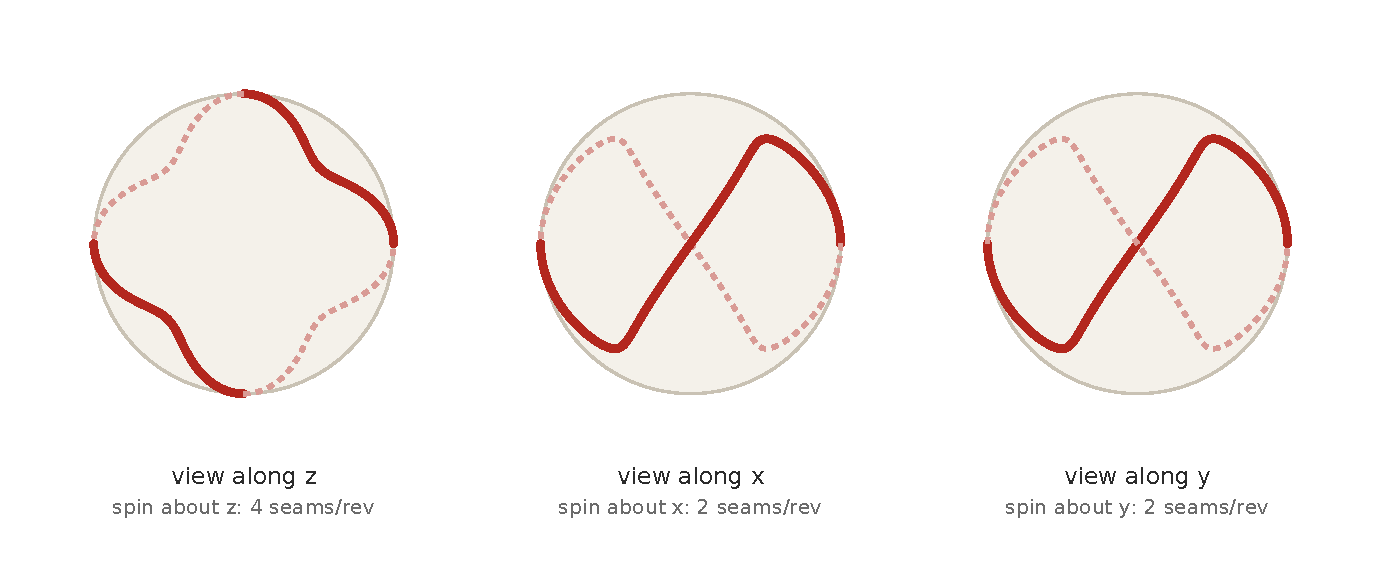
\includegraphics[width=0.95\textwidth]{figure/seam.pdf}
	\caption{パラメトリック縫い目モデル（\(A=0.7\)）の3方向からの投影。実線が手前，破線が奥。\texttt{scripts/plot\_seam.jl}で再生成できる。}
	\label{fig:seam}
\end{figure}

\paragraph{断面形状}
縫い目曲線を中心線とする半径 \(h\) の円管とする。中心線が球面上にあるため，管は球面から外側へちょうど \(h\) だけ隆起する。高さは実測値に基づき既定0.79\,mmとする。

\paragraph{符号付き距離関数（SDF）化}
球と縫い目チューブの和集合の符号付き距離関数として実装する（\texttt{src/geometry/sdf.jl}）：\(\min(\text{球のSDF}, \text{チューブのSDF})\) で評価する。これは固体外部では厳密な距離，内部では保守的な下界となるが，境界処理が必要とするのは外部側の距離のみであるため問題にならない。格子上への事前計算では，縫い目の寄与が効く表面近傍のみ（既定で表面から \(h+3\Delta x\) 以内）で縫い目距離を評価し，遠方は球のSDFで済ませる。

\subsection{移動境界の境界条件}

球は角速度 \(\vec\omega\) で自転する。密結合方式（\secref{coupling}）では計算領域はボールに追従する並進座標系に固定されるため，境界条件としては「その場での自転」のみを扱えばよく，並進運動はフレーム側で吸収される。

\begin{itemize}
	\item \textbf{基本手法}：補間バウンスバック法（Bouzidi/Yu型 interpolated bounce-back）を用い，格子点と実際の球面（縫い目を含む）との交点位置に応じてサブグリッド精度で反射則を補間する。
	\item \textbf{表面速度条件}：境界上の各点で \(\vec u_{wall}=\vec\omega\times\vec r\) を課し，回転による運動量を流体側へ正しく伝達する。
\end{itemize}

\subsection{力・トルクの評価}

球表面上の運動量交換則（Momentum Exchange Method, MEM）により，格子ボルツマンの粒子分布から直接，球に働く圧力抵抗・摩擦抵抗・揚力・トルクを運動量収支として算出する。これにより解析式に頼らず，流体場から一貫して瞬時の \(\vec F_{aero}\)，\(\vec T_{aero}\) を得る。

\subsection{回転する縫い目球と局所再カット}
\label{sec:recut}

回転境界条件は \(\vec u_{wall}=\vec\omega\times\vec r\) を課すが，これは滑面球には十分でも縫い目球には足りない——球は回しても同じ形だが，縫い目球は向きによって形が変わる。しかも縫い目は到達可能などの解像度でもサブセル（1格子間隔未満）の特徴であるため（\secref{resolution-budget}），ソルバから見た「縫い目」の実体は補間バウンスバックの距離パラメータ \(\delta\) そのものである。\(\delta\) を固定したままでは，静止した模様を着た滑面球を解いていることになる。

ボール追従座標系ではボールは並進せず，かつ球は回転対称であるため，分類が変わりうる節点の集合は向きによらない薄いシェルに固定される：球の内部（\(\varphi_{sphere}<0\)）は縫い目チューブが和集合として加わるだけなので常に固体，球面から十分離れた外側（\(\varphi_{sphere}>h+\sqrt3\)）はチューブの隆起もバウンスバックのリンクも届かないため常に流体である。その間だけがシェルであり，再カット（自転に伴う固体・流体分類の更新）の対象となる。境界節点の列番号は初期化時に一度だけ割り当てられ，再カットは値の上書きのみで完結する。

縫い目の対称性（\(u\to u+\pi\)すなわち\(z\)軸まわり\(180^\circ\)回転で自己一致）を用いた検証では，その向きでの再カット結果が元のカットとビット単位で一致することを確認しており，探索・シェル番号付け・二分法のいずれもこの対称性を壊していないことの強い証拠となっている。

再カットが必要な頻度は，1ステップあたりの赤道での表面移動量（格子間隔単位）
\begin{align}
	\omega\,\Delta t\,\frac{R}{\Delta x} = \frac{\omega R}{U}\,u_{lattice} = S\,u_{lattice}
	\label{eq:recut-rate}
\end{align}
から決まり，\(\Delta x\)に依存しない——\textbf{スピンパラメータと格子マッハ数だけで決まる}。本プロジェクトの検証ケース（\(S=0.272\)，\(u_{lattice}=0.05\)）では0.0136格子/ステップであり，1/4格子ごとに再カットするなら18ステップおきでよい。これが密結合ループ（\secref{coupling-loop}）のサブサイクル長の上限を決める。


\newpage
\section{密結合方式による軌道計算}
\label{sec:coupling}

\subsection{方式の選定}

検討したいピッチ条件は少数（数条件程度）であるため，軌道再現の忠実度を優先し，係数テーブルによる補間方式（疎結合方式）ではなく，\textbf{CFDと運動方程式を毎ステップ結合する密結合方式}を採用する。少数条件のみを高精度に再現したい場合，密結合方式のコストは疎結合方式の2--3倍程度に留まる一方，条件数が数十を超える多条件スタディでは疎結合方式が圧倒的に有利になる（\(10^4\)条件規模で約200倍のコスト差）。将来的に多条件のパラメトリックスタディが必要になった場合は，疎結合方式への切り替えを推奨する。

\subsection{ボール追従座標系（非慣性系）}
\label{sec:frame}

密結合とは，マウンドからホームベースまでの約18.4\,m（ボール約400個分）を実空間で移動格子等により直接解くことを意味しない——単一のコンシューマGPU（8\,GB VRAM）でこれを行うのは非現実的である。そこで\textbf{ボール追従非慣性座標系（body-fitted moving reference frame）}を採用し，計算領域自体はボール周囲数直径角の小さな箱に保ったまま，実時間で運動方程式と結合する。

\begin{enumerate}
	\item 計算領域はボールの重心を原点とする座標系に固定する（ボールは領域内で自転するのみで並進しない）。
	\item 流入境界条件は，その瞬間のボールの対気速度ベクトル \(-\vec V_{ball}(t)\) に相当する一様流として毎ステップ更新する。
	\item 座標系が加速度運動（重力による落下，抗力による減速）をしているため，非慣性系補正として一様体積力（見かけの重力項）をLBMのフォーシング項に追加し，流体側の運動量収支を物理的に正しく保つ。
	\item 各タイムステップ（またはサブサイクルごと）で運動量交換法（\secref{geometry-boundary}）により瞬時の \(\vec F_{aero}\)，\(\vec T_{aero}\) を算出し，6自由度運動方程式（\eref{translation}, \eref{rotation}）に代入してその場でRK4により時間積分する。
	\item 更新された対気速度・角速度を，次ステップの流入境界条件・体積力・自転境界条件へフィードバックする。
\end{enumerate}

この構成により，係数テーブルを介さずCFDと運動方程式が毎ステップ双方向に結合された「真の密結合」でありながら，計算領域を小さな箱に保てるため，単一の8\,GB級GPUでも実行可能になる。

\subsection{見かけの体積力の導出}
\label{sec:apparent-force}

フレームはボールと同じ加速度
\begin{align}
	\vec A = \frac{d\vec V}{dt} = \frac{\vec F_{aero}}{m} + \vec g
	\label{eq:frame-accel}
\end{align}
で運動するため，流体の運動方程式には一様な見かけの力 \(-\rho\vec A\) が加わる。一方，実際の重力 \(+\rho\vec g\) は，静止大気中では静水圧勾配と釣り合っているため，両方とも落とすことと両方とも持つことが等価である（差は浮力のみで，野球ボールでは2.6\,mN対自重1.42\,N＝0.18\%）。したがって流体が受ける一様体積加速度は
\begin{align}
	\vec a_{fluid} = -\vec A = -\left(\frac{\vec F_{aero}}{m} + \vec g\right)
	\label{eq:apparent-force}
\end{align}
となり，\textbf{重力は流体側には直接現れない}（ボールの応答を通してのみ流れ場に効く）。自由落下（\(\vec F_{aero}=0\)）では \(\vec a_{fluid}=-\vec g\)，すなわち空気が上向きに \(g\) で加速して見える，という直感とも一致する。

この形が本質的に重要なのは，次の恒等式が成り立つためである。フレームから見た主流速度は \(\vec u_\infty=-\vec V(t)\) であり，
\begin{align}
	\frac{d\vec u_\infty}{dt} = -\vec A = \vec a_{fluid}.
	\label{eq:identity}
\end{align}
つまり\textbf{フレームの加速度を表す体積力そのものが，遠方場を次ステップの流入条件が要求する速度へちょうど運ぶ}。境界条件と内部場が食い違って静かに破綻する，という移動座標系スキームの典型的な失敗モードが構造的に起きない。

6自由度側（並進・自転・姿勢）では，姿勢はジンバルロック（スピン軸が飛行方向に近づくジャイロ成分の強い変化球で現実的な危険）を避けるため四元数で保持し，積分にはRK4を用いる。CFDから凍結した力を与える限り，並進・自転についてRK4は厳密である。

\subsection{密結合ループとサブサイクル平均}
\label{sec:coupling-loop}

密結合ループの1回の外側反復は次の4段からなる：

\begin{enumerate}
	\item 箱平均速度を測り体積力（\eref{apparent-force}）を決める。
	\item サブサイクル分だけLBMを進め，運動量交換の力をその区間で平均する。
	\item 力・トルクをN・N\(\cdot\)mに変換し，6自由度運動方程式を1ステップ進める。
	\item 更新された速度・角速度を(1)へ戻す。
\end{enumerate}

\paragraph{サブサイクルの目的は省力化ではなく平均化である}
ボールの速度は1球（約\(1.85\times10^5\)ステップ）で15\%しか変わらない——1ステップあたり\(10^{-6}\)——であり，軌道側は毎ステップの更新を必要としない。一方，乱流中の物体に働く瞬時の運動量交換力は平均値より大きく揺らぐため，区間平均でなければ軌道に与える標本として不適切である。

\paragraph{力の使い方に一貫性が要る}
同一ステップ内では，直前のサイクルで測った力を体積力にも6自由度積分にも使う。\eref{identity}の恒等式が項ごとに成立するのは，フレーム加速度を表す力とボールを加速する力が\emph{同じ数値}であるときだけである。新しく測った力を軌道に，前サイクルの力を流体に使うと，遠方場と流入条件が1サイクル分ずれる。

\subsection{力の分解}

各サブサイクルで運動量交換の力を \((\hat u,\hat n,\hat b)\) 系に分解して記録する：\(\hat u=\vec V/|\vec V|\)（抗力方向），\(\hat n=(\vec\omega\times\hat u)/|\vec\omega\times\hat u|\)（マグヌス方向。飛行方向成分のスピン＝ジャイロ成分は構成上自動的に落ちる），\(\hat b=\hat u\times\hat n\)。第3成分 \(C_{side}\) が本プロジェクトの要点である（\secref{magnus}）：実球は縫い目がマグヌス面まわりの圧力分布を非対称にするためこの方向に力を持ち，それがスウィーパーやジャイロボールが教科書どおりに曲がらない主因である。解析的な係数モデルはここに必ずゼロを返すが，CFDは測った値を返せる。

\subsection{流入・流出境界条件}
\label{sec:open-boundary}

計算領域を単純な周期境界とした場合，ボールは自分自身の後流の中を飛ぶことになる。抗力係数の基準とすべき「球に届く流れ」が周期箱では曖昧になり，その曖昧さが本来測ろうとしている物理量の差より大きくなりうることが検証（\secref{validation}）で判明したため，流れ方向の面だけを非周期の流入・流出境界に置き換える機能を実装した（\texttt{src/boundary/open.jl}）。

流れ方向は \(-x\) 方向であるため，高\(x\)面が入口，低\(x\)面が出口となる。いずれもGuoの非平衡外挿を用い，内側の第1平面から非平衡部 \(f^{neq}\) を持ってくる：

\begin{itemize}
	\item \textbf{入口}：速度を課し，密度は内側から取る。自由流を「推定」せず「指定」する。
	\item \textbf{出口}：密度を課し，速度は内側から取る。後流が対流で流出し，圧力の基準がここで固定される。
\end{itemize}

分担が逆だと成立しない。出口が圧力を固定しないと箱全体の密度が漂い，入口が密度まで課すと過剰決定になって条件が跳ね返る。

流入・流出境界を導入すると，周期境界で必要だった平均流コントローラ（\secref{controller}）は不要になる——入口があれば自由流を直接指定でき，ボール追従座標系では\eref{identity}の恒等式が「内部の流体は入口値と同じ率で加速する」ことを保証するので，フィードバックそのものが要らない。

\subsection{平均流コントローラ（周期境界での暫定措置）}
\label{sec:controller}

流入・流出境界を用いない構成（完全周期境界）では，球が受ける抗力の分だけ流体の運動量が行き場を失い，主流が減衰する。そこで箱平均速度を目標値 \(-\vec V(t)\) に保つ一様体積力を加える（constant-mass-flux forcing）。

このコントローラはPI制御でなければならない。純積分制御では誤差が \(\ddot e=-Ke\) に従い減衰しないため体積力が目標値のまわりで振動するが，目標値自体が極めて小さい（定常補正は1サブサイクルあたり平均速度を0.03\%程度動かす量）ため，わずかな振動でも信号が埋もれてしまう。比例項を加えて \(K_p=2/T\)，\(K_i=1/T^2\)（臨界減衰）とすると運動量収支の残差は実用的な水準に収まる。ここで \(T\) は箱の通過時間の数倍にとる。

定常状態では，コントローラが供給する運動量と表面から運動量交換法で得た力が一致しなければならない（フレームの体積力は\eref{identity}の恒等式により相殺して現れない）。この2つはまったく別経路で計算されるため，両者の残差は強制項・境界条件・単位換算のすべてが整合していることの常時チェックとして使える。

この構成には既知の限界がある：周期像によるブロッケージは残るため，領域幅を十分にとる必要がある。検証（\secref{validation}）により，この限界は想定より重いことが定量的に判明している。


\newpage
\section{GPU実装}
\label{sec:gpu}

\subsection{想定ハードウェアとデータレイアウト}

本プロジェクトは単一のコンシューマGPU（NVIDIA GeForce RTX 3060 Ti，VRAM 8\,GB GDDR6）を実行環境として想定する。LBMはメモリ帯域律速のアルゴリズムであるため，実効性能はデータセンター向けGPUよりも一桁近く低く，8\,GBのVRAMが格子点数の上限を決める最大の制約となる。

実装言語はJuliaとし，GPUカーネルはCUDA.jlを用いて直接記述する。データレイアウトはSoA（Structure of Arrays）とし，分布関数 \(f_i\) を速度方向ごとに連続配列として保持することでメモリコアレッシングを最大化する。

\subsection{AA-pattern（in-place streaming）}

8\,GB VRAMという制約を踏まえ，AA-pattern（in-place streaming）を採用する（\texttt{src/core/aa\_pattern.jl}）。通常のping-pong方式（2バッファ）に対し，分布関数のメモリフットプリントを約半減できる：D3Q27・FP32では\(27\times4=108\,\text{byte}\)/ノードとなり，本番解像度（\(320^3\)）で約3.6\,GB。ping-pong方式なら約7.1\,GBとなり8\,GBのカードには収まらないため，この選択は必須である。

実装ではD3Q27を「立方体スロット順」で保持する：スロット \(s\) と速度 \(\vec c\) の対応を
\begin{align}
	c = \left((s-1)\bmod3,\ \left\lfloor\frac{s-1}{3}\right\rfloor\bmod3,\ \left\lfloor\frac{s-1}{9}\right\rfloor\right) - (1,1,1)
	\label{eq:cube-slot}
\end{align}
に固定することで，速度・重み・反対方向がすべて整数演算で求まり（反対スロットは\(28-s\)），カーネル内でのテーブル参照が不要になる。またAAパターンでは2つのノードが同じスロットに触れないため，スレッド間の競合が原理的に発生しない。

AAパターンで8ステップ進めた結果は，既存の2格子方式（解析解で検証済み）と相対誤差\(10^{-12}\)で一致することをBGK・中心モーメント両方で確認している。

\subsection{解像度とVRAMの見積り}
\label{sec:resolution-budget}

AA-pattern・D3Q27・FP32を前提に，1格子点あたりの必要メモリを見積もる。分布関数27方向で\(27\times4=108\,\text{byte}\)，固体フラグ等の付随データを含めて概算130--140\,byte程度になる。RTX 3060 Ti（8\,GB）のうちOS等のオーバーヘッドを見込み計算に使えるVRAMを約7\,GBと仮定すると，格子点数の上限は概ね\(5\times10^7\)点程度となる。

\begin{table}[H]
	\centering
	\caption{一様格子（立方体領域，N点/D）における解像度とコストの関係。}
	\label{tab:resolution-budget}
	\begin{tabular}{cccccccc}
		\Hline{1.5pt}
		N/D & L/D & 一辺 & VRAM & \(\Delta x\) (mm) & 縫い目/\(\Delta x\) & 境界層/\(\Delta x\) & 時間 \\
		\hline
		40  & 8 & 320 & 3.42\,G & 1.870 & \textbf{0.42} & 0.40 & 0.7\,h \\
		50  & 6 & 300 & 2.82\,G & 1.496 & 0.53 & 0.51 & 0.8\,h \\
		60  & 6 & 360 & 4.87\,G & 1.247 & 0.63 & 0.61 & 1.6\,h \\
		80  & 4 & 320 & 3.42\,G & 0.935 & 0.84 & 0.81 & 1.5\,h \\
		120 & 3 & 360 & 4.87\,G & 0.623 & 1.27 & 1.21 & 3.2\,h \\
		\hline
	\end{tabular}
\end{table}

\textbf{縫い目高さと境界層厚は同じ数字である。} 代表条件（\(U=39\,\text{m/s}\)）の赤道位置での層流境界層厚は\(5\sqrt{\nu x/U}\approx0.76\,\text{mm}\)であり，縫い目高さ0.79\,mmと5\%以内で一致する。粗さ要素が境界層と同程度の高さを持つことは，それが遷移を誘発するトリップとして働く条件そのものであり（\secref{aerodynamics}），同時に「縫い目を解像すること」と「境界層を解像すること」が2つの独立な要求ではなく1つであることを意味する。\tabref{resolution-budget}の縫い目/\(\Delta x\)列と境界層/\(\Delta x\)列が常に一緒に動くのはこのためである。

一様格子で領域を8Dに保つ限り，VRAM上限内で到達できる解像度は縫い目高さの0.42セル程度にとどまる。1セル以上に載せるには領域を3D程度まで狭めるしかないが，そこでは球が箱の1/6を占め，これはブロッケージ（\secref{validation}のHasimoto解比較で定量化した周期像の影響）そのものが無視できない大きさになってしまう。この一様格子の限界が，局所グリッドリファインメント（\secref{grid-refinement}）を最適化ではなく必須要件として位置づける根拠である。1レベル・2倍細分化の導入により，同じ8D領域・同程度のVRAMで縫い目解像度をおよそ2倍にできることを確認している。

\subsection{壁面境界のGPU実装}

融合カーネル（衝突・体積力・ストリーミングを1カーネルに融合したもの）では，バウンスバックを読み出し側ではなく\emph{書き出し側}に置く。書き出しの時点でスレッドは自ノードの衝突後分布を保持しており，それがバウンスバックに必要なものそのものだからである。跳ね返った値は，次のステップで自分自身が読みに来るスロットへ直接書き込む：偶数ステップで固体へ向かう方向 \(s\) は隣接固体ノードのスロットへ，奇数ステップでは自ノードの反対スロット \(28-s\) へ書く。これにより読み出し側には壁面の処理が一切不要になり，スレッド間の競合が生じないというAAパターンの性質もそのまま保たれる。跳ね返り値が同じステップ・同じノードの衝突後分布と密度から作られるため，2格子方式の参照実装と項ごとに一致し，近似ではなく厳密な比較ができる（分布関数で相対誤差\(10^{-12}\)，力・トルクで\(10^{-10}\)の一致を確認済み）。

境界ノードは自身の通し番号を持つため，各ノードが専用の列に力・トルクを書き出し，後段で総和を取る。アトミック演算は不要であり，2つのスレッドが同じ列に触れることもない。

この方式の制約として，Bouzidiの \(\delta<1/2\) 分岐は「1つ外側の流体ノードの衝突後分布」を必要とするが，融合カーネルのスレッドはそれを持たない。該当リンクはハーフウェイ規則にフォールバックする（\(\delta\ge1/2\)は自ノードの分布のみで済むため補間規則を使う）。2格子方式側にも同じ規則を用意してあるため参照実装と厳密に一致し，この妥協のコストは推測ではなく測定できる。

\subsection{局所グリッドリファインメント}
\label{sec:grid-refinement}

\subsubsection{音響スケーリング}

細分化比 \(m\) の局所グリッドリファインメントでは，時間刻み \(\Delta t\) を空間刻み \(\Delta x\) と一緒に半分にする（音響スケーリング）。時間刻みを両レベルで共通にすれば界面の時間補間が不要になり実装は大幅に楽になるが，その場合物理音速 \(c_{phys}=\Delta x/(\Delta t\sqrt3)\) が粗細で異なることになり，音波が界面でインピーダンス不整合を起こして部分反射する。移動境界は音響ノイズを出し続けるため，これを細格子内に閉じ込める必要がある。

\begin{table}[H]
	\centering
	\caption{細分化比 \(m\) に対する物理量のスケーリング。添字 c/f は粗/細格子を表す。}
	\label{tab:acoustic-scaling}
	\begin{tabular}{lll}
		\Hline{1.5pt}
		量 & 関係 & 理由 \\
		\hline
		緩和時間 & \(\tau_f-1/2=m(\tau_c-1/2)\) & \(\nu_{lat}=\nu\,\Delta t/\Delta x^2\) が \(m\) 倍 \\
		体積加速度 & \(a_f=a_c/m\) & \(a\propto\Delta t^2/\Delta x\) \\
		ひずみ速度 & \(S_f=S_c/m\) & \(S_{lat}=S_{phys}\Delta t\) \\
		格子速度・マッハ数 & 不変 & 音響スケーリングの定義 \\
		\hline
	\end{tabular}
\end{table}

非平衡部の再スケールは特に間違えやすい。分布関数はそのままでは移せない：平衡分布 \(f^{eq}\) は \(\rho,u\)のみに依存し，音響スケーリングはこれらを変えないためそのまま渡るが，非平衡部 \(f^{neq}\) はひずみ速度を担うため渡らない。Chapman-Enskog展開より \(f^{neq}\propto\tau_{lat}S_{lat}\) なので
\begin{align}
	\alpha \equiv \frac{f^{neq}_{fine}}{f^{neq}_{coarse}}
	= \frac{\tau_f}{m\,\tau_c}
	= \frac{\tau_f(\tau_c-1/2)}{\tau_c(\tau_f-1/2)}.
	\label{eq:alpha}
\end{align}
\(\alpha\)は\(\tau\)に依存する定数ではない——\(\tau\to1/2\)で\(1/m\)に，\(\tau\)が大きいと\(1\)に近づく。したがって\(\tau\)によらない式を用いると，投球レイノルズ数が強いる緩和時間域でちょうど\(m\)倍近く外れる一方，\(\tau\approx1\)のベンチマークでは数十\%の差にしか見えず離散化誤差と紛れる。

\subsubsection{配置と検証結果}

細格子は粗格子インデックスの範囲を覆う直方体パッチとし，一辺は\(2(\text{範囲})+1\)節点になるよう配置する。奇数インデックスが粗格子節点と一致し偶数が中間になるため，粗→細の転送に一般の補間は不要で，1・2・4・8点の平均で済む。1サイクルは粗2ステップ・細4ステップ（AAパターンの偶数レイアウトに両レベルが揃って戻る単位）である。

\begin{table}[H]
	\centering
	\caption{2格子リファインメントの検証結果。}
	\label{tab:refine-validation}
	\begin{tabular}{lc}
		\Hline{1.5pt}
		項目 & 結果 \\
		\hline
		一様流の転送（両方向） & 厳密（\(3\times10^{-18}\) / \(6\times10^{-17}\)） \\
		一様流の1サイクル（BGK） & 厳密（\(<10^{-14}\)） \\
		物理ひずみ速度の保存（粗↔細） & 相対\(10^{-11}\)以内 \\
		Taylor-Green渦の収束次数（音響スケーリング） & \textbf{1.98 / 2.42} \\
		\hline
	\end{tabular}
\end{table}

パッチ形状については，物体に沿った形（球殻など）ではなく軸並行の直方体を採用している。物体適合形状が有利に見えるのは節点数だけであり（同じ幅の球は立方体の52\%の体積），この節約は密な直方体配列から間接参照（索引付きリスト）へ格納形式を変えたときにのみ実体化する。実測した索引アクセスの帯域は直接コピーの0.11倍（局所性が最悪の場合）であり，実行全体で見込める節約の上限は11.7\%程度に対し，悪化の下限が4.8倍という非対称な結果から，直方体パッチを採用している。加えて，物体に密着した界面は剥離せん断層——本プロジェクトが最も精度を必要とする領域——の内部に置かれてしまうため，精度の観点からも直方体形状（界面を穏やかな流れの中に置く）が優れている。

パッチのアスペクト比については，ボールを中心とする立方体は前方の助走と後方の後流に同じ長さを割り当てるが，前方の流れは半径の半分も行けば滑らかである一方，後方の剥離とせん断層はどのレイノルズ数でもそれより長く伸びる。そこで各パッチを下流側にのみ延長するオプション（\texttt{--refine-wake}）を設けている。

\subsection{性能実測}

RTX 3060 Ti上での実測MLUPS（Mega Lattice Update Per Second）を示す。

\begin{table}[H]
	\centering
	\caption{精度・衝突演算子別の実測性能（周期境界のみ）。}
	\label{tab:mlups}
	\begin{tabular}{llrr}
		\Hline{1.5pt}
		精度 & 衝突演算子 & 実測MLUPS & 実効メモリ帯域 \\
		\hline
		FP32 & 中心モーメント & 2{,}544 & 549\,GB/s \\
		FP32 & BGK & 2{,}563 & 554\,GB/s \\
		FP64 & BGK & 246 & 106\,GB/s \\
		FP64 & 中心モーメント & 215 & 93\,GB/s \\
		\hline
	\end{tabular}
\end{table}

FP32ではカーネルはメモリ帯域に完全に張り付いている——BGKと中心モーメントが同一の性能を示すこと自体が帯域律速の証拠であり（演算量の差が性能に現れない），実測帯域（549--554\,GB/s）は同カードでの単純コピーベンチの実測帯域（513--532\,GB/s）とほぼ一致する。したがって，これ以上の高速化にはメモリトラフィック自体を減らす以外に手段がない。

一方，FP64は演算律速である（このカードのFP64は1/64レート）。BGKの方が中心モーメントより速いという順序が，演算律速であることを裏付けている。速度差が12倍あり，かつTaylor-Green渦での粘性再現はFP32でも誤差\(-0.06\%\)と精度上の問題がないため，本番計算はFP32とする。

壁面境界を含むカーネルの実測では，周期境界のみの場合に対する速度低下は3\%未満に留まる。境界に触れる節点が全体の1\%程度しかないうえ，バウンスバックを書き出し側に置いたことでギャザー側に壁の分岐が一切入らず，力・トルクのリダクションもアトミック操作を使わずに済むためである。

以上より，本番構成（8D領域・40点/D，\(320^3\)格子）での1条件あたりの計算時間は
\begin{align}
	\frac{3.28\times10^7\ \text{点}\times3.7\times10^5\ \text{ステップ}}{2.56\times10^9\ \text{更新/秒}} \approx 4.8\times10^3\ \text{秒} \approx \textbf{1.3時間/条件}
	\label{eq:runtime-estimate}
\end{align}
と見積もられる。これは計画段階の概算（15--20時間/条件）の約1/13であり，この余裕は解像度およびグリッドリファインメントに充てている。


\newpage
\section{検証（Validation \& Verification）}
\label{sec:validation}

少数条件を高忠実度で解く密結合方式では，各本番実行の信頼性を事前にどれだけ担保できるかが重要になる。本章では，段階的な検証計画とその結果を要約する。

\subsection{V\&V-1：コード基礎検証}

層流Poiseuille流，Taylor-Green渦など解析解を持つベンチマークで，LBM実装の収束次数を確認した。減衰Taylor-Green渦（3次元格子にz方向一様で埋め込んだ2次元渦）で，実効動粘性が\eref{viscosity}と一致すること（運動エネルギー減衰率から逆算して誤差2\%以内），速度場が解析解と2\%以内で一致すること（相対L2誤差，\(n=32\)，200ステップ），空間収束次数が設計どおり2次精度（\(n=16/32/64\)で2.03/1.94，\(\tau=0.8\)）であることを確認した。

\(\tau\)を\(1/2\)近傍（例：0.55）に取ると，BGKの高次誤差項が2次項と同程度になり測定次数が1.3--1.8へ乱れることも確認しており，収束次数の検証は\(\tau=0.8\)程度の条件で行う必要がある。

\subsection{V\&V-2：乱流モデル検証（クリープ流極限）}

周期立方配列中の球（\(a/L=1/6\)）に体積力を与え，定常状態の抗力をHasimotoの解析解と比較した。レイノルズ数を一定（\(\approx0.03\)）に保ち解像度のみを変えたところ，補間バウンスバック＋厳密な\(\delta\)評価では，実測抗力/Hasimoto予測の比が半径4--8格子で0.958--0.974と，解像度とともに単調に1へ近づくことを確認した。定常状態での運動量収支（壁への力／体積力の総和）は全ケースで0.9999以上であり，力の算出そのものが正しいことも確認済みである。

\subsection{V\&V-2：乱流モデル検証（高レイノルズ数側）}
\label{sec:validation-highre}

一様流中の滑面球についてClift-Gauvin相関との比を測定した。当初，周期境界のみの構成では，低レイノルズ数域で比が0.5未満と大きく外れる現象が見られた。詳細な切り分けの結果，これは離散化誤差ではなく\emph{周期境界による後流の巻き込み}が原因であることが判明した：周期箱では球に届く流れが箱平均速度の31\%程度しかなく，抗力係数の基準速度が大きく過大評価されていた。

\subsubsection{流入・流出境界の導入とその効果}

\secref{open-boundary}の流入・流出境界を導入し，同じ条件（\(Re=100\)，N/D=20，横幅4D）で再測定したところ，球に届く流れは入口指定値の96.4\%まで回復し，Clift-Gauvin比は0.47から1.12（相関自身の不確かさの範囲内）まで改善した。幅を無限大へ線形外挿すると，比は\textbf{1.012}に収束する。この結果により，\(Re=100\)におけるV\&V-2は合格と判断した。

\subsubsection{壁面条件の検証}

流入・流出境界のもとで，領域幅・バウンスバック規則・緩和時間をそれぞれ独立に変えて壁面条件の妥当性を検証した。

\begin{table}[H]
	\centering
	\caption{バウンスバック規則の比較（幅4D，Clift-Gauvin比）。\(\tau\)・Ma・Re・N/Dはすべて同一で，壁位置のみが異なる。}
	\label{tab:bounceback-rule}
	\begin{tabular}{lcc}
		\Hline{1.5pt}
		規則 & N/D=20 & N/D=40 \\
		\hline
		補間バウンスバック & 1.12 & 1.09 \\
		ハーフウェイ & 1.16 & 1.11 \\
		\hline
		規則差 & 3.5\% & \textbf{1.8\%} \\
	\end{tabular}
\end{table}

規則差は\(\Delta x\)を半分にすると半減しており，壁位置の1次の離散化誤差として設計どおり収束している。この結果に基づき，補間バウンスバック規則を採用した。

中心モーメント演算子では，3次以上のキュムラントの緩和率が2次モーメントのそれと独立に選べるため，TRTのmagic parameter \(\Lambda=(1/\omega^+-1/2)(1/\omega^--1/2)\)を自由に設定できる（\secref{cumulant}）。ポアズイユ流の速度分布から実効壁位置を放物線フィットで取り出して測定したところ，既定値 \(\omega^-=1\) が実質的に最適であり，\(\Lambda\)をTRTの理論値\(3/16\)（壁を格子の中間に置くとされる値）に強制すると，むしろ壁位置は数倍悪化することを確認した。この結果は，壁面条件が\(Re=100\)で観測される緩和時間依存性（後述）の原因ではないことを示す独立した証拠になっている。

\subsubsection{緩和時間依存性の切り分け}

流入・流出境界のもとでも，緩和時間 \(\tau\) を振ると抗力比が7\%程度動く現象が残った。これに対し，圧縮性（\(Ma^2\)），壁面条件（上述），解像度で消える打ち切り誤差，数値粘性の下限，単精度の丸め誤差という5つの仮説を，いずれも「動かせば動くはずのものを動かして，動かなかった」形で個別に検証し，すべて棄却した。原因は未特定のまま残っているが，Clift-Gauvin相関自身の不確かさとV\&V-5の許容誤差（後述，変化量20\%）を踏まえ，この6\%程度の緩和時間依存性はコード全体の不確かさとして申告した上で本番実行に進む方針とした。なお本番の\(\tau-1/2\)は，この検証で振った範囲よりもさらに一桁以上\(1/2\)に近い領域にある。

\subsection{V\&V-2：局所グリッドリファインメントの直接検証}

外側領域・ボール・タイムステップ数を揃え，一様な細格子とリファインド格子で力を比較した。

\begin{table}[H]
	\centering
	\caption{一様細格子とリファインド格子の抗力・揚力の比較。}
	\label{tab:refine-drag}
	\begin{tabular}{lrr}
		\Hline{1.5pt}
		構成 & 抗力 & 揚力 \\
		\hline
		一様細格子（基準） & \(-0.5975\) & 0.01527 \\
		リファインド，パッチ3.5D & \(-0.5905\)（\(-1.2\%\)） & 0.01467（\(-4.0\%\)） \\
		リファインド，パッチ2.5D & \(-0.6240\)（\(+4.4\%\)） & 0.01633（\(+6.9\%\)） \\
		\hline
	\end{tabular}
\end{table}

パッチが十分大きければ（本プロジェクトでは3直径以上），リファインド格子は一様細格子を数\%以内で再現する。狭いパッチが外れるのは，界面がボール表面から近い位置に来て，粗レベルが表現できない近傍後流をそこで課すことになるためである。

\subsection{V\&V-3：回転球検証}

滑面回転球のマグヌス係数について，\(S<0.4\)の範囲で\(C_L\approx S\)の線形関係を再現することを確認する（実施予定）。CPU参照実装では，無回転で横力・トルクが機械精度でゼロになること，マグヌス力の向きが\(\vec\omega\times\hat V\)と一致しスピン反転に対して反対称であること，流体が自転を引き戻す向きのトルクが出ることを確認済みである。

\subsection{V\&V-4：縫い目球検証}

縫い目付き球体を固定・一様流中に置いた場合の\(C_D\)，\(C_L\)を実測データ\cite{kensrud2010thesis,nathan2008}と比較し，縫い目向き依存性・非マグヌス力の再現性を確認する（実施予定）。密結合ループの助走・スピンアップ段階を流用できる。

\subsection{V\&V-5：軌道検証}
\label{sec:vv5}

既知の実測ピッチトラッキングデータと，密結合シミュレーションの軌道出力を比較する。検証ケースとして，WBC2023決勝，大谷翔平の対トラウト最終球（2023年3月21日，9回裏2死フルカウント）を採用した\cite{cbssports2023,si2023}。

\begin{table}[H]
	\centering
	\caption{V\&V-5検証ケースの実測値。}
	\label{tab:vv5-case}
	\begin{tabular}{ll}
		\Hline{1.5pt}
		項目 & 実測値 \\
		\hline
		球種（Statcast分類） & スウィーパー \\
		球速 & 87.2\,mph（\(\approx38.99\,\text{m/s}\)） \\
		スピン量 & 2708\,rpm \\
		横変化量 & 17\,in（\(\approx0.432\,\text{m}\)） \\
		縦変化量 & 32\,in（\(\approx0.813\,\text{m}\)） \\
		\hline
	\end{tabular}
\end{table}

球速・回転数はシミュレーションの初期条件として直接使用し，横変化量・縦変化量をシミュレーション軌道から同一定義で算出した値と比較することで合格基準とする。ただし，スピン軸の正確な向き（チルト角・ヨー角）とリリースポイント座標は本稿執筆時点で未確認であり，別途確認またはキャリブレーションで補う必要がある。

\paragraph{「変化量」の定義について}
「変化量」は単一の軌道の性質ではなく2本の軌道の差であり，どちらを基準に取るかで値が2倍近く変わる。この差は許容誤差（暫定20\%）よりはるかに大きいため，比較の前に定義を確定させる必要がある。実装では3つの定義（pfx：本塁手前40\,ft地点で分岐しマグヌス力のみ切った軌道，induced：リリース時点から分岐した同様の軌道，total：無力の直進基準）をすべて算出し，報告値がどの定義と対応するかを明示的に比較できるようにしている。


\newpage
\section{まとめと今後の課題}

本ノートでは，格子ボルツマン法による変化球軌道シミュレーションの理論的背景（\secref{aerodynamics}--\secref{turbulence}）と実装方法（\secref{geometry-boundary}--\secref{gpu}），および検証結果（\secref{validation}）をまとめた。現時点で得られている主要な結論は次のとおりである。

\begin{itemize}
	\item 中心モーメント衝突演算子と\(\omega_{odd}\)/\(\omega_{higher}\)の分離により，本番レイノルズ数（\(\sim2\times10^5\)）で必要な緩和時間域でも数値的に安定な計算が可能であることを確認した。
	\item 周期境界における後流の巻き込みが，高レイノルズ数側のV\&V-2で見られた大きな誤差の主因であることを特定し，流入・流出境界の導入によってこれを解消した。
	\item 壁面条件（補間バウンスバック，実効壁位置）は複数の独立な検証により系統誤差が無いことを確認した一方，緩和時間に依存する6\%程度の誤差の原因は本稿執筆時点では未特定であり，コードの不確かさとして申告した上で本番実行に進んでいる。
	\item AA-pattern・局所グリッドリファインメント・GPU実装により，1条件あたりの計算時間を計画段階の見積り（15--20時間）から約1.3時間まで短縮した。
\end{itemize}

\subsection{今後の課題}

\begin{itemize}
	\item \textbf{緩和時間依存性の原因特定}：\secref{validation-highre}で残った6\%の緩和時間依存性について，曲面壁での補間バウンスバックと運動量交換法の組み合わせに特有の効果である可能性が高く，平板壁での検証（本稿の壁面条件の検証）だけでは十分条件になっていない。
	\item \textbf{グリッドリファインメントの多段化}：現状は1レベル・2倍細分化のみが実装されている。縫い目を1格子間隔以上で解像するには，細格子内へのさらなる入れ子（2レベル目）が必要である。
	\item \textbf{V\&V-3・V\&V-4の実施}：回転滑面球のマグヌス係数検証，および縫い目付き球体の固定・一様流中での検証を完了させる。
	\item \textbf{V\&V-5の実施}：スピン軸の向き・リリースポイントの確認またはキャリブレーション，「変化量」の定義の確定を経て，WBC2023決勝の検証ケースで本番実行と実測比較を行う。
	\item \textbf{可視化パイプラインの拡充}：解析モデル軌道の対話的可視化（段階1）は実装済みであり，CFD軌道の同様の可視化（段階2）が残っている。
\end{itemize}

本ノートは開発の進行に伴って随時更新する予定であり，日々の検証結果や設計判断のより詳細な記録は，本リポジトリの設計ノート（\texttt{docs/design/DESIGN.md}）を参照されたい。


\newpage
\bibliographystyle{junsrt}
\bibliography{ref}

\end{document}
